\documentclass[a4paper,11pt,exos]{nsi} % COMPILE WITH DRAFT
\usepackage{pifont}
\usepackage{fontawesome5}
\geometry{margin=2cm}




\begin{document}
\classe{\terminale Comp}
\titre{Corrigé de l'évaluation-bilan 3}
\maketitle

\exo{}
\begin{enumerate}
    \item \textcolor{UGLiBlue}{Soit $f$ la fonction définie sur $I=\fif{0}{12}$ par $\quad f(x)=2xe^{-x}$.}
    \begin{enumalph}
        \item \textcolor{UGLiBlue}{Démontrer que pour tout $x\in I, \quad f'(x)=2(1-x)e^{-x}$.}\\[.5em]
        Soit $x\in\fif{0}{12}$ 
        \begin{tabbing}
            $f'(x)$ \= $=2e^{-x}+2x\times (-1)e^{-x}$\\
            \> $=2e^{-x}-2xe^{-x}$\\
            \> $=2(1-x)e^{-x}$
        \end{tabbing}

        \item \textcolor{UGLiBlue}{Dresser le tableau de variations de la fonction $f$ sur $I=\fif{0}{12}$.}\\[.5em]
        Pour tout $x\in\fif{0}{12}$, $e^{-x}>0$, donc $f'(x)$ est du signe de $(1-x)$.\\
        On a $\quad f(0)=0$ ; $\quad f(1)=e^{-1}\approx 0,74\quad$ et $\quad f(12)=24e^{-12}\approx 0,0001$.\\
        \begin{center}
            \begin{tikzpicture}
            \tkzTabInit[color,lgt=3,espcl=3]
            {$x$/.7,signe de $f'(x)$ /.7,variations de $f$ /2}
            {$0$,$1$, $12$}
            \tkzTabLine{,+,z,-,}
            \tkzTabVar{-/$0$,+/$2e^{-1}$,-/$24e^{-12}$}
            \end{tikzpicture}
            \end{center}
            
        \item \textcolor{UGLiBlue}{Démontrer que l'équation $f(x)=0,2$ admet deux solutions sur l'intervalle $I$.\\
        Donner, à l'aide de la calculatrice, une valeur approchée au centième de chacune de ces solutions.}\\[.5em]
        Sur l'intervalle $\fif{0}{1}$, la fonction $f$ est continue et strictement croissante.\\
        De plus $f(0)=0<0,2$ et $f(1)=e^{-1}>0,2$, donc d'après le théorème des valeurs intermédiaires pour les fonctions strictement monotones, l'équation $f(x)=0,5$ admet une unique solution sur l'intervalle $\fif{0}{1}$.\\
        Sur l'intervalle $\fif{1}{12}$, la fonction $f$ est continue et strictement décroissante.\\
        De plus $f(1)=e^{-1}>0,2$ et $f(12)=24e^{-12}<0,2$, donc d'après le théorème des valeurs intermédiaires pour les fonctions strictement monotones, l'équation $f(x)=0,5$ admet une unique solution sur l'intervalle $\fif{1}{12}$.\\
        On en déduit que la fonction $f$ admet (exctement) deux solutions $\alpha_1$ et $\alpha_2$ sur l'intervalle $I$.\\
        À l'aide de la calculatrice, on trouve $\alpha_1\approx 0,11$ et $\alpha_2\approx 3,57$.
    \end{enumalph}
   
    \item \textcolor{UGLiBlue}{Le taux d'alcoolémie d'une personne pendant les 12 heures qui suivent la consommation d'une certaine quantité d'alcool est modélisé par la fonction $f$.
    \begin{enumerate}[label=\textbullet]
        \item $x$ représente le temps écoulé (en heures) depuis la consommation d'alcool.
        \item $f(x)$ représente le taux d'alcoolémie (en grammes par litre de sang).
    \end{enumerate}}
    \begin{enumalph}
        \item \textcolor{UGLiBlue}{Décrire les variations du taux d'alcoolémie de cette personne pendant les 12 heures suivant la consommation d'alcool.}\\[.5em]
        La première heure, le taux d'alcoolémie augmente. Il diminue ensuite les 11 heures suivantes.
        \item \textcolor{UGLiBlue}{À quel moment le taux d'alcoolémie de cette personne est-il maximal ? Quelle est alors sa valeur ? Arrondir au centième.}\\[.5em]
        Le taux d'alcoolémie est maximal à l'instant où la fonction $f$ admet un maximum. Le tableau de variations de la fonction $f$ montre que le maximum est atteint en $x=1$.\\
        Cela signifie que le taux d'alcoolémie est maximal une heure après la consommation d'alcool.\\
        Sa valeur est $f(1)=e^{-1}$ soit environ 0,74 g/L.
        \item \textcolor{UGLiBlue}{Le code de la route fixe le taux d'alcoolémie maximal autorisé à 0,2 g/L pour les jeunes conducteurs. Combien de temps après la consommation d'alcool cette personne jeune conductrice est-elle autorisée à prendre le volant ? Donner la réponse en heures et minutes.}\\[.5em]
        On cherche à résoudre l'inéquation $f(x)\leqslant 0,2$.\\
        D'après la question \textbf{1.c.}, on sait que l'ensemble des solutions de cette inéquation est la réunion des intervalles $\fif{0}{\alpha_1}$ et $\fif{\alpha_2}{12}$.\\
        La personne peut donc prendre le volant environ 3,57 heures soit 3 heures et 34 minutes après la consommation d'alcool.
    \end{enumalph}  
\end{enumerate}

\exo{}
\textcolor{UGLiBlue}{Un supermarché souhaite acheter des pommes à un fournisseur qui propose des prix au kilogramme dégressifs en fonction de la masse commandée.\\
Pour une commande de $x$ kilogrammes de pommes, le prix $p(x)$, en euros, pour un kilogramme de fruit est donné par :
$$ p(x)=\dfrac{x+300}{x+100}\quad \text{pour }x\in\fio{100}{+\infty}.$$}
\subsection*{Partie A : Étude du prix $p$ proposé par le fournisseur}
\begin{enumerate}
    \item \textcolor{UGLiBlue}{Montrer que pour tout $x\in\fio{100}{+\infty}, \quad p(x)=\dfrac{1+\dfrac{300}{x}}{1+\dfrac{100}{x}}$.}
    \begin{tabbing}
         Soit $x\in\fio{100}{+\infty}$, on a :$\quad p(x)$ \= $=\dfrac{x+300}{x+100}$\\[.5em]
        \> $=\dfrac{x\left(1+\dfrac{300}{x}\right)}{x\left(1+\dfrac{100}{x}\right)}$\\[.5em]
        \> $=\dfrac{1+\dfrac{300}{x}}{1+\dfrac{100}{x}}$
    \end{tabbing}
    \item \textcolor{UGLiBlue}{En déduire la limite de la fonction $p$ en $+\infty$.}\\[.5em]
    On a $\quad\lim\limits_{x\to+\infty}\dfrac{300}{x}=0\quad$ et $\quad\lim\limits_{x\to+\infty}\dfrac{100}{x}=0$.\\
    Donc $\lim\limits_{x\to+\infty}p(x)=\dfrac{1+0}{1+0}=1$.
    \item \textcolor{UGLiBlue}{Calculer $p'(x)$ pour tout $x\in\fio{100}{+\infty}$ puis dreser le tableau de variations de la fonction $p$.}\\[.5em]
    Soit $x\in\fio{100}{+\infty}$, on a :
    \begin{tabbing}
        $p(x)=\dfrac{u(x)}{v(x)}\quad$ avec \quad \=$u(x)=x+300\quad$ et \quad \=$v(x)=x+100$.\\
        \>  $u'(x)=1$ \> $v'(x)=1$.
    \end{tabbing}
    \begin{tabbing}
        $p'(x)$ \= $=\dfrac{u'(x)v(x)-u(x)v'(x)}{\left(v(x)\right)^2}$\\[.5em]
        \> $=\dfrac{(x+100)-(x+300)}{(x+100)^2}$\\[.5em]
        \> $=\dfrac{-200}{(x+100)^2}$
    \end{tabbing}
    Ainsi, pour tout $x\in\fio{100}{+\infty}$, $p'(x)<0$.\\
    La fonction $p$ est donc strictement décroissante sur $\fio{100}{+\infty}$.
    \begin{center}
        \begin{tikzpicture}
        \tkzTabInit[color,lgt=3,espcl=3]
        {$x$/.7,signe de $p'(x)$ /.7,variations de $p$ /2}
        {$100$, $+\infty$}
        \tkzTabLine{,-,}
        \tkzTabVar{+/$2$,-/$1$}
        \end{tikzpicture}
    \end{center}
    \item \textcolor{UGLiBlue}{Interpréter économiquement les variations de la fonction $p$.}\\[.5em]
    Plus la quantité de pommes commandée est importante, plus le prix au kilogramme est faible. Le prix maximal est de 2 euros pour un kilogramme de pommes, il est atteint pour une commande de 100 kilogrammes. La limite du prix est de 1 euro pour un kilogramme de pommes.
\end{enumerate}

\subsection*{Partie B : Étude de la somme à dépenser}
\begin{enumerate}
    \item \textcolor{UGLiBlue}{Quelle somme devra dépenser le supermarché pour acheter à ce fournisseur 150 kilogrammes de pommes ? 700 kilogrammes de pommes ?}\\[.5em]
    Pour 150 kilogrammes de pommes, le prix est de $p(150)=\dfrac{150+300}{150+100}=\dfrac{450}{250}=1,80$ euros par kilogramme.\\
    Donc le supermarché devra dépenser $150\times 1,80=270$ euros.\\[.5em]
    Pour 700 kilogrammes de pommes, le prix est de $p(700)=\dfrac{700+300}{700+100}=\dfrac{1000}{800}=1,25$ euros par kilogramme.\\
    Donc le supermarché devra dépenser $700\times 1,25=875$ euros.
    \item \textcolor{UGLiBlue}{On appelle $S(x)$ la somme, en euros, que le supermarché devra dépenser pour acheter $x$ kilogrammes de pommes vendues au prix de $p(x)$ euros par kilogramme.}
    \begin{enumalph}
        \item \textcolor{UGLiBlue}{Par définition, $S(x)=xp(x)$. Déterminer la limite de la fonction $S$ en $+\infty$.}\\[.5em]
        Soit $x\in\fio{100}{+\infty}$, on a :
        \begin{tabbing}
            $S(x)$ \= $=xp(x)$\\
            \> $=x\times\dfrac{x+300}{x+100}$\\[.5em]
            \> $=\dfrac{x^2+300x}{x+100}$\\[.5em]
            \> $=\dfrac{x^2\left(1+\dfrac{300}{x}\right)}{x\left(1+\dfrac{100}{x}\right)}$\\[.5em]
            \> $=\dfrac{x\left(1+\dfrac{300}{x}\right)}{1+\dfrac{100}{x}}$
        \end{tabbing}
        Or $\quad\lim\limits_{x\to+\infty}1+\dfrac{300}{x}=1\quad$ d'où $\lim\limits_{x\to+\infty}x\left(1+\dfrac{300}{x}\right)=+\infty$.\\
        De plus $\quad\lim\limits_{x\to+\infty}1+\dfrac{100}{x}=1$.\\[.5em]
        Donc par quotient de limites, on a $\lim\limits_{x\to+\infty}S(x)=+\infty$.
        \item \textcolor{UGLiBlue}{Calculer $S'(x)$ puis dresser le tableau de variations de la fonction $S$ sur $\fio{100}{+\infty}$.}\\[.5em]
        Soit $x\in\fio{100}{+\infty}$, on a :
        \begin{tabbing}
            $S(x)=\dfrac{u(x)}{v(x)}\quad$ avec \quad \=$u(x)=x^2+300x\quad$ et \quad \=$v(x)=x+100$.\\
            \>  $u'(x)=2x+300$ \> $v'(x)=1$.
        \end{tabbing}
        \begin{tabbing}
            Donc $\quad S'(x)$ \= $=\dfrac{u'(x)v(x)-u(x)v'(x)}{\left(v(x)\right)^2}$\\[.5em]
            \> $=\dfrac{(2x+300)(x+100)-(x^2+300x)}{(x+100)^2}$\\[.5em]
            \> $=\dfrac{2x^2+500x+30\ 000-x^2-300x}{(x+100)^2}$\\[.5em]
            \> $=\dfrac{x^2+200x+30\ 000}{(x+100)^2}$\\[.5em]
        \end{tabbing}
        $S'(x)$ est du signe de $x^2+200x+30000$.\\
        Calculons le discriminant de ce trinôme : $\Delta=200^2-4\times 30\ 000=40\ 000-120\ 000=-80\ 000<0$.\\
        Donc pour tout $x\in\fio{100}{+\infty}$, $S'(x)$ est du signe du coefficient dominant du polynôme $x^2+200x+30\ 000$.\\
        On a donc $S'(x)>0$ pour tout $x\in\fio{100}{+\infty}$.\\
        \begin{center}
            \begin{tikzpicture}
            \tkzTabInit[color,lgt=3,espcl=3]
            {$x$/.7,signe de $S'(x)$ /.7,variations de $S$ /2}
            {$100$, $+\infty$}
            \tkzTabLine{,+,}
            \tkzTabVar{-/$200$,+/$+\infty$}
            \end{tikzpicture}
        \end{center}
    \end{enumalph}
    \item \textcolor{UGLiBlue}{Le magasin dispose d'un budget de 900 euros pour acheter des pommes. Quelle masse maximale de pommes pourra-t-il acheter chez ce fournisseur ?}\\[.5em]
    On cherche à résoudre l'équation $S(x)\leqslant 900$.\\
    Soit $x\in\fio{100}{+\infty}$.
    \begin{tabbing}
        $S(x)\leqslant 900$ \= $\iff \dfrac{x^2+300x}{x+100}\leqslant 900$\\[.5em]
        \>  $\iff x^2+300x\leqslant 900(x+100)$\\[.5em]
        \> $\iff x^2+300x\leqslant 900x+90\ 000$\\[.5em]
        \> $\iff x^2-600x-90\ 000\leqslant 0$
    \end{tabbing}
    On calcule le discriminant de ce trinôme : $\Delta=600^2-4\times1\times (-90\ 000)=360\ 000+360\ 000=720\ 000$.\\
    On calcule les racines de ce trinôme :\\[.5em]
    $x_1=\dfrac{600-\sqrt{720\ 000}}{2}\approx -124\quad$ et $\quad x_2=\dfrac{600+\sqrt{720\ 000}}{2}\approx 724$.\\   

    On a donc le tableau de signe suivant :
    \begin{center}
        \begin{tikzpicture}
        \tkzTabInit[color,lgt=6,espcl=3]
        {$x$/.7,signe de $x^2-600x-90\ 000$ /1}
        {$100$, $x_2$, $+\infty$}
        \tkzTabLine{,-,z,+,}
        \end{tikzpicture}
    \end{center}
    Le magasin pourra donc acheter au maximum 724 kilogrammes de pommes chez ce fournisseur.
\end{enumerate}

\end{document}